%++++++++++++++++++++++++++++++++++++++++
% Don't modify this section unless you know what you're doing!
\documentclass[letterpaper,12pt]{article}
\usepackage{tabularx} % extra features for tabular environment
\usepackage{amsmath}  % improve math presentation
\usepackage{graphicx} % takes care of graphic including machinery
\usepackage[margin=1in,letterpaper]{geometry} % decreases margins
\usepackage{cite} % takes care of citations
\usepackage[final]{hyperref} % adds hyper links inside the generated pdf file
\hypersetup{
	colorlinks=true,       % false: boxed links; true: colored links
	linkcolor=blue,        % color of internal links
	citecolor=blue,        % color of links to bibliography
	filecolor=magenta,     % color of file links
	urlcolor=blue         
}
%++++++++++++++++++++++++++++++++++++++++


\begin{document}

\title{COMP 512 Phase 1 Report}
\author{Yiwei Xia and Marie Payne}
\date{\today}
\maketitle

\section{Introduction}

The goal of our project is to design and develop a distributed system where clients can make requests and servers deliver responses based upon them, with the use of a middleware server. The aim is to develop this system using two protocols, remote method invocation and through transmission control protocol (TCP).

\section{Theory}
Remote method invocation is defined as one object calling the method of another object potentially located on a remote machine (e.g. usually not local). In RMI architecture, the sender on host A invokes the method B.function(x,y) which is typically the proxy method of the local proxy object (the interface with which A can use to call methods of B). This then gets sent to the RMI layer. The method is packaged into a message (commonly a TCP/UDP packet) to be transmitted over the network to the host machine B. B processes it through the RMI layer and executes the method with the specified parameters (if given), and returns the output to A if it produced any. By using the library java.rmi.Remote, any object that extends it becomes an object that can be used and accessed remotely. The invoker object machine maintains a remote object lookup proxy table, which stores a remote object reference and a real object reference. When the method invocation is transmitted to the server (in this case, host B which is executing the method request from host A, the client), it looks up a the corresponding local object reference that calls the real object. When a remote object reference arrives in a reply message to the client, it looks up the proxy object (interface) to confirm the correct format. \\

The implementation of Remote Method Invocation is to declare the remote interfaces being implemented, so that the remote objects can be called without knowing the implementation ahead of time. A constructor must be defined for the remote object, so that it can be instantiated. The server must contain an implementation of each remote method in the remote object, which is made available to the RMI runtime environment, so that it will be processed through the RMI registry and made available to any potential clients. To call the remote object the hostname of where the object resides must be known, so that its RMIRegistry can be referenced. \\

RMI client-server architecture can be paired with a  middleware server setup to achieve a total distributed information system. The communication middleware server is what any potential client applications communicate with, and all remote method invocations are passed through this server and distributed to the corresponding resource manager server applications to be executed. The middleware server contains some functionality and can process minimal requests to lower overhead costs, however the bulk of the computation is performed on the resource manager servers' side. The following figure demonstrates this architecture, taken from Tanenbaum's Distributed Systems: Principles and Paradigms$.^{[1]}$


\begin{figure}[ht] 
	% read manual to see what [ht] means and for other possible options
	\centering 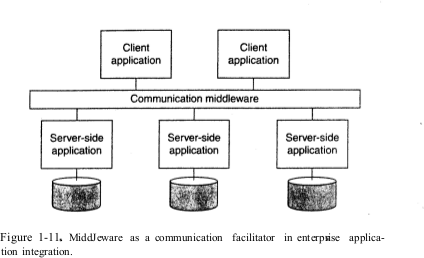
\includegraphics[width=0.8\columnwidth]{figure1.png}
	% note that in above figure file name, "sr_setup",
	% the file extension is missing. LaTeX is smart enough to find
	% apropriate one (i.e. pdf, png, etc.)
	% You can add this extention yourself as it seen below
	% both notations are correct but above has more flexibility
	%\includegraphics[width=1.0\columnwidth]{sr_setup.pdf}

\end{figure}

The Transmission Control Protocol (TCP) is a blocking, connection-oriented, reliable communication protocol which is established on the handshaking protocol and relies on input/output buffers at both ends of the communication channel. The protocol executes based on FIFO delivery principles and acknowledgement packets to provide reliability of the messages being transmitted. The client machine and server machine first transmit handshaking packets to determine that the communication channel is reliable and the hosts are as they declare themselves to be. TCP uses a sequence number on each packet so that they are guaranteed to be transmitted in the correct order, and that the message doesn't be corrupted or duplicated along the network. Acknowledgement packets or acks are sent after every message is received, to confirm transmission (message delivery guarantee). A checksum field is also included in the message to verify the message's contents. The following figure demonstrates the TCP protcol between an example client machine and several servers, processed through a switch (or middleware server)$.^{[1]}$\\


In Java, messages can be passed through TCP by using streams of data transmitted over sockets. This also allows objects/methods to be passed over client and server machines, so that objects and methods can be remotely accessed and executed. These streams can be in in XML or JSON, for easy read/write capabilities.

\begin{figure}[ht] 
	% read manual to see what [ht] means and for other possible options
	\centering 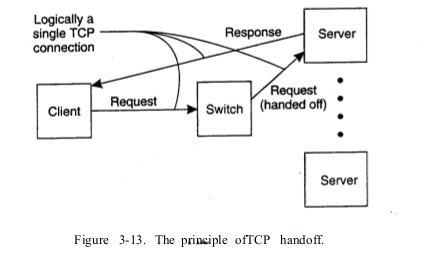
\includegraphics[width=0.8\columnwidth]{figure2.png}
	% note that in above figure file name, "sr_setup",
	% the file extension is missing. LaTeX is smart enough to find
	% apropriate one (i.e. pdf, png, etc.)
	% You can add this extention yourself as it seen below
	% both notations are correct but above has more flexibility
	%\includegraphics[width=1.0\columnwidth]{sr_setup.pdf}
	
\end{figure} 

\section{Design}

We implemented the RMI middleware server by extending the resource manager class, so that the middleware server is technically a fully functioning resource manager server with added functionality. The ports for the RM servers for each resource (car, flight, hotel rooms, customers) are hard-coded. The RM servers are considered and instantiated as clients on the middleware end, and communicated with under that assumption. The RM servers directly trasmit back to the clients. \\

We implemented the TCP middleware server by considering each of the resource manager servers as clients. The middleware, clients, and resource manager servers are run as threads with a hardcoded socket number (the Runner classes). The clients instantiate an input/output stream and connect through the middleware server's thread. The data is passed as JSON to be parsed. Using threads for each connection allows the possibility of multiple clients to use the resources, each with blocking functionality. \\

\section{Conclusion}

Distributing the servers and server requests is a very efficient way to model client-server architecture. The use of the middleware server facilitates this process and provides concurrency to the system. 

\section{Bibliography}

All the theory in this report came directly from the lecture slides on the course website or the recommended textbook, Distributed Systems: Principles and Paradigms by Andrew S. Tanenbaum and Maarten Van Steen, Second Edition, Pearson and Prentice Hall, Amsterdam, 2007. 

\end{document}